\section{Basic Principles}
\label{Basic Principles}

This section covers general principles that should be kept in mind when writing
any suite. More advanced topics are covered later: {\em Efficiency And
Maintainability} (section~\ref{Efficiency And Maintainability}) and {\em
Portable Suites} (section~\ref{Portable Suites}).

\subsection{UTC Mode}

Cylc has full timezone support if needed, but real time NWP suites should use
UTC mode to avoid problems at the transition between local standard time and
daylight saving time, and to enable the same suite to run the same way in
different timezones.

\lstset{language=suiterc}
\begin{lstlisting}
[cylc]
    UTC mode = True
\end{lstlisting}
\subsection{Fine Or Coarse-Grained Suites}

Suites can have many small simple tasks, fewer large complex tasks, or anything
in between. A task that runs many distinct processes can be split into many
distinct tasks. The fine-grained approach is more transparent and it allows
more task level concurrency and quicker failure recovery - you can rerun just
what failed without repeating anything unnecessarily.

\subsubsection{rose bunch}

One caveat to our fine-graining advice is that submitting a large number of
small tasks at once may be a problem on some platforms. If you have many
similar concurrent jobs you can use \lstinline=rose bunch= to pack them into a
single task with incremental rerun capability: retriggering the task will rerun
just the component jobs that did not successfully complete earlier.

\subsection{Monolithic Or Interdependent Suites}
\label{Monolithic Or Interdependent Suites}

When writing suites from scratch you may need to decide between putting
multiple loosely connected sub-workflows into a single large suite, or
constructing a more modular system of smaller suites that depend on each other
through inter-suite triggering. Each approach has its pros and cons, depending
on your requirements and preferences with respect to the complexity and
manageability of the resulting system.

The \lstinline=cylc gscan= GUI lets you monitor multiple suites at a time, and
you can define virtual groups of suites that collapse into a single state
summary.

\subsubsection{Inter-Suite Triggering}

A task in one suite can explicitly trigger off of a task in another suite. The
full range of possible triggering conditions is supported, including custom
message triggers. Remote triggering involves repeatedly querying (``polling'')
the remote suite run database, not the suite daemon, so it works even if the
other suite is down at the time.

There is special graph syntax to support triggering off of a task in another
suite, or you can call the underlying \lstinline=cylc suite-state= command
directly in task scripting.

In real time suites you may want to use clock-triggers to delay the onset of
inter-suite polling until roughly the expected completion time of the remote
task.

\subsection{Self-Contained Suites}
\label{Self-Contained Suites}

All files generated by Cylc during a suite run are confined to the {\em suite
run directory} \lstinline=$HOME/cylc-run/<SUITE>=. However, Cylc has no control
over the locations of the programs, scripts, and files, that are executed,
read, or generated by your tasks at runtime.  It is up to you to ensure that
all of this is confined to the suite run directory too, as far as possible.

Self-contained suites are more robust, easier to work with, and more portable.
Multiple instances of the same suite (with different suite names) should be
able to run concurrently under the same user account without mutual
interference.

\subsubsection{Avoiding External Files}

Suites that use external scripts, executables, and files beyond the essential
system libraries and utilities are vulnerable to external changes: someone
else might interfere with these files without telling you.

In some case you may need to symlink to large external files anyway, if space
or copy speed is a problem, but otherwise suites with private copies of all the
files they need are more robust.

\subsubsection{Installing Files At Start-up}

Use \lstinline=rose suite-run= {\em file creation mode} or \lstinline=R1=
install tasks to copy files to the self-contained suite run directory at
start-up.  Install tasks are preferred for time-consuming installations because
they don't slow the suite start-up process, they can be monitored in the GUI,
they can run directly on target platforms, and you can rerun them later without
restarting the suite. 

\subsubsection{Confining Ouput To The Run Directory}

Output files should be confined to the suite run directory tree. Then all
output is easy to find, multiple instances of the same suite can run
concurrently without interference, and other users should be able to copy and
run your suite with few modifications. Cylc provides a \lstinline@share@
directory for generated files that are used by several tasks in a suite
(see~\ref{Shared Task IO Paths}). Archiving tasks can use \lstinline=rose arch=
to copy or move selected files to external locations as needed (see~\ref{Suite
Housekeeping}).

\subsection{Task Host Selection}

At sites with multiple task hosts to choose from, use
\lstinline=rose host-select= to dynamically select appropriate task hosts
rather than hard coding particular hostnames. This enables your suite to
adapt to particular machines being down or heavily overloaded by selecting
from a group of hosts based on a series of criteria.
\lstinline=rose host-select= will only return hosts that can be contacted by
non-interactive SSH.

\subsection{Task Scripting}

Non-trivial task scripting should be held in external files rather than
inlined in the suite.rc. This keeps the suite definition tidy, and it
allows proper shell-mode text editing and independent testing of task scripts.

For automatic access by task jobs, task-specific scripts should be kept in 
Rose app bin directories, and shared scripts kept in (or installed to) the
suite bin directory.

\subsubsection{Coding Standards}

When writing your own task scripts make consistent use of appropriate coding
standards such as:

\begin{itemize}
    \item PEP8 for Python - \url{https://www.python.org/dev/peps/pep-0008/}
    \item Google Shell Style Guide for Bash -
      \url{https://google.github.io/styleguide/shell.xml}
\end{itemize}

\subsubsection{Basic Functionality}

In consideration of future users who may not be expert on the internals of your
suite and its tasks, all task scripts should:

\begin{itemize}
  \item Print clear usage information if invoked incorrectly (and via the
    standard options \lstinline=-h, --help=).
  \item Print useful diagnostic messages in case of error. For example, if a
    file was not found, the error message should contain the full path to the
    expected location.
  \item Always return correct shell exit status - zero for success, non-zero
    for failure. This is used by Cylc job wrapper code to detect success and
    failure and report it back to the suite daemon.
  \item In shell scripts use \lstinline=set -u= to abort on any reference to
    an undefined variable. If you really need an undefined variable to evaluate
    to an empty string, make it explicit: \lstinline@FOO=${FOO:-}@.
  \item In shell scripts use \lstinline=set -e= to abort on any error without
      having to failure-check each command explicitly.
\end{itemize}


\subsection{Rose Apps}

Rose apps allow all non-shared task configuration - which is not relevant to
workflow automation - to be moved from the suite definition into app config
files. This makes suites tidier and easier to understand, and it allows
\lstinline=rose edit= to provide a unified metadata-enhanced view of the suite
and its apps (see~\ref{Rose Metadata Compliance}).

Rose apps are a clear winner for tasks with complex configuration requirements.
It matters less for those with little configuration, but for consistency and to
take full advantage of \lstinline=rose edit= it makes sense to use Rose apps
for most tasks.

When most tasks are Rose apps, set the app-run command as a root-level default,
and override it for the occasional non Rose app task:

\lstset{language=suiterc}
\begin{lstlisting}
[runtime]
    [[root]]
        script = rose task-run -v
    [[rose-app1]]
        #...
    [[rose-app2]]
        #...
    [[hello-world]]  # Not a Rose app.
        script = echo "Hello World"
\end{lstlisting}

\subsection{Rose Metadata Compliance}
\label{Rose Metadata Compliance}
 
Rose metadata drives page layout and sort order in \lstinline=rose edit=, plus
help information, input validity checking, macros for advanced checking and app
version upgrades, and more.

To ensure the suite and its constituent applications are being run as intended
it should be valid against any provided metadata: launch the
\lstinline=rose edit= GUI or run \lstinline=rose macro --validate= on the
command line to highlight any errors, and correct them prior to use. If errors
are flagged incorrectly you should endeavour to fix the metadata.

When writing a new suite or application, consider creating metadata to
facilitate ease of use by others.

\subsection{Task Independence}

Essential dependencies must be encoded in the suite graph, but tasks should
not
rely unnecessarily on the action of other tasks. For example, tasks should
create their own output directories if they don't already exist, even if they
would normally be created by an earlier task in the workflow. This makes it is
easier to run tasks alone during development and testing.


\subsection{Clock-Triggered Tasks}
\label{Clock-Triggered Tasks}
Tasks that wait on real time data should use clock-triggers to delay job
submission until the expected data arrival time:

\lstset{language=suiterc}
\begin{lstlisting}
[scheduling]
    initial cycle point = now
    [[special tasks]]
        # Trigger 5 min after wall-clock time is equal to cycle point.
        clock-trigger = get-data(PT5M)
    [[dependencies]]
        [[[T00]]]
            graph = get-data => process-data
\end{lstlisting}

Clock-triggered tasks typically have to handle late data arrival. Task
execution {\em retry delays} can be used to simply retrigger the task at
intervals until the data is found, but frequently retrying small tasks probably
should not go to a batch scheduler, and multiple task failures will be logged
for what is a essentially a normal condition (at least it is normal until the
data is really late).

Rather than using task execution retry delays to repeatedly trigger a task that
checks for a file, it may be better to have the task itself repeatedly poll for
the data (see~\ref{Rose App File Polling} for example).

\subsection{Rose App File Polling}
\label{Rose App File Polling}

Rose apps have built-in polling functionality to check repeatedly for the
existence of files before executing the main app. See the \lstinline=[poll]=
section in Rose app config documentation. This is a good way to implement
check-and-wait functionality in clock-triggered tasks (\ref{Clock-Triggered
Tasks}), for example.

It is important to note that frequent polling may be bad for some filesystems,
so be sure to configure a reasonable interval between polls. 

\subsection{Task Execution Time Limits}

Instead of setting job wall clock limits directly in batch scheduler
directives, use the \lstinline=execution time limit= suite config item.
Cylc automatically derives the correct batch scheduler directives from this,
and it is also used to run \lstinline=background= and \lstinline=at= jobs via
the \lstinline=timeout= command, and to poll tasks that haven't reported in
finished by the configured time limit.

\subsection{Restricting Suite Activity}
\label{Restricting Suite Activity}

It may be possible for large suites to overwhelm a job host by submitting too
many jobs at once:

\begin{itemize}
  \item Large suites that are not sufficiently limited by real time clock
      triggering or inter-cycle dependence may generate a lot of {\em runahead}
      (this refers to Cylc's ability to run multiple cycles at once, restricted
      only by the dependencies of individual tasks).
  \item Some suites may have large families of tasks whose members all
    become ready at the same time.
\end{itemize}

These problems can be avoided with {\em runahead limiting} and {\em internal
queues}, respectively.

\subsubsection{Runahead Limiting}
\label{Runahead Limiting}

By default Cylc allows a maximum of three cycle points to be active at the same time, but this value is configurable:

\lstset{language=suiterc}
\begin{lstlisting}
[scheduling]
    initial cycle point = 2020-01-01T00
    # Don't allow any cycle interleaving:
    max active cycle points = 1
\end{lstlisting}

\subsubsection{Internal Queues}

Tasks can be assigned to named internal queues that limit the number of members
that can be active (i.e.\ submitted or running) at the same time:

\lstset{language=suiterc}
\begin{lstlisting}
[scheduling]
    initial cycle point = 2020-01-01T00
    [[queues]]
        # Allow only 2 members of BIG_JOBS to run at once:
        [[[big_jobs_queue]]]
            limit = 2
            members = BIG_JOBS
    [[dependencies]]
        [[[T00]]]
            graph = pre => BIG_JOBS
[runtime]
    [[BIG_JOBS]]
    [[foo, bar, baz, ...]]
        inherit = BIG_JOBS
\end{lstlisting}

\subsection{Suite Housekeeping}
\label{Suite Housekeeping}

Ongoing cycling suites can generate an enormous number of output files and logs
so regular housekeeping is very important. Special housekeeping tasks,
typically the last tasks in each cycle, should be included to archive selected
important files and then delete everything at some offset from the current
cycle point.

The Rose built-in apps \lstinline=rose_arch= and \lstinline=rose_prune=
provide an easy way to do this. They can be configured easily with
file-matching patterns and cycle point offsets to perform various housekeeping
operations on matched files.

\subsection{Complex Jinja2 Code}

The Jinja2 template processor provides general programming constructs,
extensible with custom Python filters, that can be used to {\em generate} the
suite definition. This makes it possible to write flexible multi-use
suites with structure and content that varies according to various input
switches. There is a cost to this flexibility however: excessive use of Jinja2
can make a suite hard to understand and maintain. It is difficult to say
exactly where to draw the line, but we recommend erring on the side of
simplicity and clarity: write suites that are easy to understand and therefore
easy to modify for other purposes, rather than extremely complicated suites
that attempt do everything out of the box but are hard to maintain and modify.

Note that use of Jinja2 loops for generating tasks is now deprecated in favour
of built-in parameterized tasks - see~\ref{Parameterized Tasks}.

\subsection{Shared Configuration}

Configuration that is common to multiple tasks should be defined in one
place and used by all, rather than duplicated in each task. Duplication is
a maintenance risk because changes have to be made consistently in several
places at once.

\subsubsection{Jinja2 Variables}

In simple cases you can share by passing a Jinja2 variable to all the tasks
that need it:

\lstset{language=suiterc}
\begin{lstlisting}

[runtime]
    [[foo]]
        script = run-foo --version={{JOB_VERSION}}
    [[bar]]
        script = run-bar --version={{JOB_VERSION}}
\end{lstlisting}

\subsubsection{Inheritance}

Sharing by inheritance of task families is recommended when more than a few
configuration items are involved.

The simplest application of inheritance is to set set global defaults in the
\lstinline=[[runtime]][root]= namespace that is inherited by all tasks.
However, this should only be done for settings that really are used
by the vast majority of tasks. Over-sharing of via root, particularly of
environment variables, is a maintenance risk because it can be very
difficult to be sure which tasks are {\em using} which global variables.

Any \lstinline=[runtime]= settings can be shared - scripting, host
and batch scheduler configuration, environment variables, and so on - from
single items up to complete task or app configurations.  At the latter extreme,
it is quite common to have several tasks that inherit the same complete
job configuration followed by minor task-specific additions:

\lstset{language=suiterc}
\begin{lstlisting}
[runtime]
    [[FILE-CONVERT]]
        script = convert-netcdf
        #...
    [[convert-a]]
        inherit = FILE-CONVERT
        [[[environment]]]
              FILE_IN = file-a
    [[convert-b]]
        inherit = FILE-CONVERT
        [[[environment]]]
              FILE_IN = file-b
\end{lstlisting}

Inheritance is covered in more detail from an efficiency perspective in
Section~\ref{The Task Family Hierarchy}.

\subsubsection{Shared Task IO Paths}
\label{Shared Task IO Paths}

If one task uses files generated by another task (and both see the same
filesystem) a common IO path should normally be passed to both tasks via a
shared environment variable. As far as Cylc is concerned this is no different
to other shared configuration items, but there are some additional aspects
of usage worth addressing here.

Primarily, for self-containment (see~\ref{Self-Contained Suites}) shared IO
paths should be under the {\em suite share directory}, the location of which is
passed to all tasks as \lstinline=$CYLC_SUITE_SHARE_PATH=.

The \lstinline@rose task-env@ utility can provide additional environment
variables that refer to static and cyclepoint-specific locations under the
suite share directory.

\lstset{language=suiterc}
\begin{lstlisting}
[runtime]
    [[my-task]]
        env-script = $(eval rose task-env -T P1D -T P2D)
\end{lstlisting}

For a current cycle point of \lstinline=20170105= this will make the following
variables available to tasks:

\lstset{language=sh}
\begin{lstlisting}
ROSE_DATA=$CYLC_SUITE_SHARE_PATH/data
ROSE_DATAC=$CYLC_SUITE_SHARE_PATH/cycle/20170105
ROSE_DATACP1D=$CYLC_SUITE_SHARE_PATH/cycle/20170104
ROSE_DATACP2D=$CYLC_SUITE_SHARE_PATH/cycle/20170103
\end{lstlisting}

Subdirectories of \lstinline@$ROSE_DATAC@ etc.\ should be agreed between
different sub-systems of the suite; typically they are named for the
file-generating tasks, and the file-consuming tasks should know to look there.

The share-not-duplicate rule can be relaxed for shared files whose names are
agreed by convention, so long as their locations under the share directory are
proper shared suite variables. For instance the Unified Model uses a large
number of files whose conventional names (\lstinline=glu_snow=, for example)
can reasonably be expected not to change, so they are typically hardwired into
app configurations (as \lstinline=$ROSE_DATA/glu_snow=, for example) to avoid
cluttering the suite definition.

Here two tasks share a workspace under the suite share directory by inheritance:

\lstset{language=suiterc}
\begin{lstlisting}
# Sharing an I/O location via inheritance.
[scheduling]
    [[dependencies]]
        graph = write_data => read_data
[runtime]
    [[root]]
        env-script = $(eval rose task-env)
    [[WORKSPACE]]
        [[[environment]]]
            DATA_DIR = ${ROSE_DATA}/png
    [[write_data]]
        inherit = WORKSPACE
        script = """
mkdir -p $DATA_DIR
write-data.exe -o ${DATA_DIR}"""
    [[read_data]]
        inherit = WORKSPACE
        script = read-data.exe -i ${DATA_DIR}
\end{lstlisting}

In simple cases where an appropriate family does not already exist paths can
be shared via Jinja variables:

\lstset{language=suiterc}
\begin{lstlisting}
# Sharing an I/O location with Jinja2.

[scheduling]
    [[dependencies]]
        graph = write_data => read_data
[runtime]
    [[write_data]]
        script = """
mkdir -p {{DATA_DIR}}
write-data.exe -o {{DATA_DIR}}"""
    [[read_data]]
        script = read-data.exe -i {{DATA_DIR}}
\end{lstlisting}

For completeness we note that it is also possible to configure multiple tasks
to use the same work directory so they can all share files in \lstinline@$PWD@.
(Cylc executes task jobs in special work directories that by default are unique
to each task). This may simplify the suite slightly, and it may be useful if
you are unfortunate enough to have executables that are designed for IO in
\lstinline@$PWD@, {\em but it is not recommended.} There is a higher risk
of interference between tasks; it will break \lstinline=rose task-run=
incremental file creation mode; and \lstinline=rose task-run --new= will in
effect delete the work directories of tasks other than its intended target.

\lstset{language=suiterc}
\begin{lstlisting}
# Shared work directory: tasks can read and write in $PWD - use with caution!
[scheduling]
    initial cycle point = 2018
    [[dependencies]]
        [[[P1Y]]]
            graph = write_data => read_data
[runtime]
    [[WORKSPACE]]
        work sub-directory = $CYLC_TASK_CYCLE_POINT/datadir
    [[write_data]]
        inherit = WORKSPACE
        script = write-data.exe
    [[read_data]]
        inherit = WORKSPACE
        script = read-data.exe
\end{lstlisting}

\subsection{Varying Behaviour By Cycle Point}

To make a cycling job behave differently at different cycle points you {\em
could} use a single task with scripting that reacts to the cycle point it finds
itself running at, but it is better to use different tasks (in different
cycling sections) that inherit the same base job configuration. This results
in a more transparent suite that can be understood just by inspecting the
graph:

\lstset{language=suiterc}
\begin{lstlisting}
# Run the same job differently at different cycle points.
[scheduling]
    initial cycle point = 2020-01-01T00
    [[dependencies]]
        [[[T00]]]
            graph = pre => long_fc => post
        [[[T12]]]
            graph = pre => short_fc => post
[runtime]
    [[MODEL]]
        script = run-model.sh
    [[long_fc]]
        inherit = MODEL
        [[[job]]]
            execution time limit = PT30M
        [[[environment]]]
            RUN_LEN = PT48H
    [[short_fc]]
        inherit = MODEL
        [[[job]]]
            execution time limit = PT10M
        [[[environment]]]
            RUN_LEN = PT12H
\end{lstlisting}

The few differences between \lstinline=short_fc= and \lstinline=long_fc=,
including batch scheduler resource requests, can be configured after common
settings are inherited.

\subsubsection{At Start-Up}

Similarly, if a cycling job needs special behaviour at the initial (or any other)
cycle point, just use a different logical task in an \lstinline=R1= graph and
have it inherit the same job as the general cycling task, not a single task
with scripting that behaves differently if it finds itself running at the
initial cycle point.

\subsection{Automating Failure Recovery}

\subsubsection{Job Submission Retries}

When submitting jobs to a remote host, use job submission retries to
automatically resubmit tasks in the event of network outages. Note this is
distinct from job retries for job execution failure (just below).

Job submission retries should normally be host (or host-group for
\lstinline=rose host-select=) specific, not task-specific, so configure them in
a host (or host-group) specific family. The following suite.rc fragment
configures all HPC jobs to retry on job submission failure up to 10
times at 1 minute intervals, then another 5 times at 1 hour intervals:

\lstset{language=suiterc}
\begin{lstlisting}
[runtime]
    [[HPC]]  # Inherited by all jobs submitted to HPC.
        [[[job]]]
            submission retry delays = 10*PT1M, 5*PT1H
\end{lstlisting}

\subsubsection{Job Execution Retries}

Automatic retry on job execution failure is useful if you have good reason to
believe that a simple retry will usually succeed. This may be the case if the
job host is known to be flaky, or if the job only ever fails for one known
reason that can be fixed on a retry. For example, if a model fails occasionally
with a numerical instability that can be remedied with a short timestep rerun,
then an automatic retry may be appropriate:

\lstset{language=suiterc}
\begin{lstlisting}
[runtime]
    [[model]]
        script = """
if [[ $CYLC_TASK_TRY_NUMBER > 1 ]]; then
    SHORT_TIMESTEP=true
else
    SHORT_TIMESTEP=false
fi
model.exe"""
        [[[job]]]
            execution retry delays = 1*PT0M
\end{lstlisting}

\subsubsection{Failure Recovery Workflows}

For recovery from failures that require explicit diagnosis you can configure
alternate routes through the workflow, together with {\em suicide triggers}
that remove the unused route. In the following example, if the model fails a
diagnosis task will trigger; if it determines the cause of the failure is a
known numerical instability (e.g.\ by parsing model job logs) it will succeed,
triggering a short timestep run. Postprocessing can proceed from either the
original or the short-step model run, and suicide triggers remove the unused
path from the workflow:

%\begin{figure}[H]
%\noindent\begin{minipage}[b]{0.65\textwidth} %
\lstset{language=suiterc}
\begin{lstlisting}
[scheduling]
    [[dependencies]]
        graph = """
            model | model_short => postproc
            model:fail => diagnose => model_short
              # Clean up with suicide triggers:
            model => ! diagnose & ! model_short
            model_short => ! model"""
\end{lstlisting}
%\end{minipage}\hfill
%\begin{minipage}[b]{0.15\textwidth}
  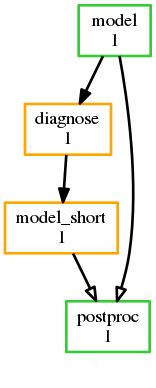
\includegraphics[width=0.18\textwidth]{resources/png/failure-recovery.png}
%\end{minipage}
%\end{figure}

\subsection{Include Files}

Include-files should not be overused, but they can sometimes be useful
(e.g.\ see Portable Suites~\ref{Portable Suites}):

\begin{lstlisting}
#...

\end{lstlisting}

(Technically this inserts a Jinja2-rendered file template). Cylc also has a
native include mechanism that pre-dates Jinja2 support and literally inlines
the include-file:

\begin{lstlisting}
#...
%include 'inc/foo.rc'
\end{lstlisting}

The two methods normally produce the same result, but use the Jinja2 version if
you need to construct an include-file name from a variable (because Cylc
include-files get inlined before Jinja2 processing is done):

\begin{lstlisting}
#...

\end{lstlisting}


